% Source: graduate-coursework/Sp26/CSCE775/course_notes/bellman_equation_guide.tex
% Description: The ``Backup'' Diagram: Average over all possible next states.

\documentclass[border=4pt]{standalone}
\usepackage{amsfonts}
\usepackage{amsmath}
\usepackage{amssymb}
\usepackage{amsthm}
\usepackage[T1]{fontenc}
\usepackage{graphicx}
\usepackage{tikz}
\usepackage{xcolor}
\usetikzlibrary{arrows.meta, positioning, shapes.geometric, calc, decorations.pathreplacing}

\definecolor{Garnet}{HTML}{73000a}
\definecolor{SecondaryBlue}{HTML}{466A9F}
\definecolor{SecondaryGreen}{HTML}{65780B}
\definecolor{FlatRed}{HTML}{CC2E40}
\definecolor{FlatDark}{HTML}{1F414D}
\definecolor{FlatYellow}{HTML}{CED318}
\definecolor{FlatGold}{HTML}{A49137}
\definecolor{LightGray}{HTML}{F0F0F0}

\renewcommand{\baselinestretch}{1.2}
\newcommand{\vocab}[1]{\textbf{\textcolor{Garnet}{#1}}}
\newcommand{\mathhighlight}[1]{\textcolor{SecondaryBlue}{#1}}

\begin{document}
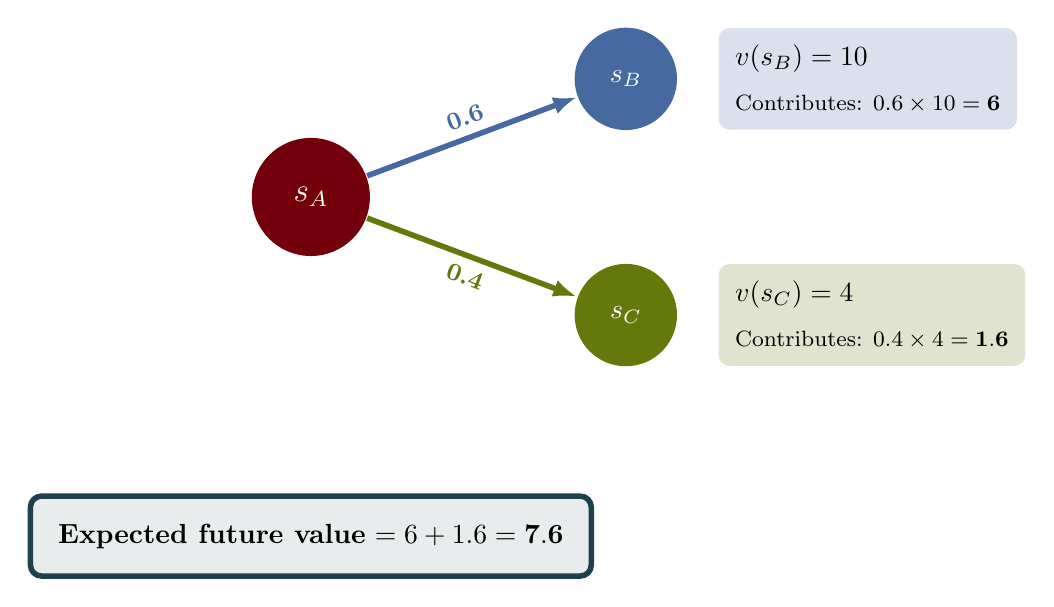
\begin{tikzpicture}[thick]
        % Current state
        \node[circle, fill=Garnet, text=white, minimum size=1.5cm, font=\large] (s) at (0,0) {$s_A$};

        % Future states
        \node[circle, fill=SecondaryBlue, text=white, minimum size=1.3cm] (s1) at (4, 1.5) {$s_B$};
        \node[circle, fill=SecondaryGreen, text=white, minimum size=1.3cm] (s2) at (4, -1.5) {$s_C$};

        % Arrows with calculations
        \draw[-{Latex[length=3mm]}, line width=2pt, SecondaryBlue] (s) -- node[above, sloped, font=\small\bfseries] {0.6} (s1);
        \draw[-{Latex[length=3mm]}, line width=2pt, SecondaryGreen] (s) -- node[below, sloped, font=\small\bfseries] {0.4} (s2);

        % Value and calculation boxes
        \node[right=0.5cm of s1, fill=SecondaryBlue!20, inner sep=6pt, rounded corners, align=left] {$v(s_B) = 10$\\[0.2em]\footnotesize Contributes: $0.6 \times 10 = \mathbf{6}$};
        \node[right=0.5cm of s2, fill=SecondaryGreen!20, inner sep=6pt, rounded corners, align=left] {$v(s_C) = 4$\\[0.2em]\footnotesize Contributes: $0.4 \times 4 = \mathbf{1.6}$};

        % Result
        \node[below=3cm of s, draw=FlatDark, line width=2pt, rounded corners, inner sep=10pt, fill=FlatDark!10] {
            \textbf{Expected future value} $= 6 + 1.6 = \mathbf{7.6}$
        };
    \end{tikzpicture}
\end{document}
